\section{Open loop analysis}

\subsection{}
Since the wind speed $\mathbf{V}_w$ is assumed zero, we have that the ground speed is
\begin{equation}\begin{aligned}
\label{eq:ground_air}
\mathbf{V}_g = \mathbf{V}_a - \mathbf{V}_w = \mathbf{V}_a.
\end{aligned}\end{equation}

\subsection{}
The definition of crab angle from REF:BEARD is
\begin{equation}\begin{aligned}
\chi_c \triangleq \chi - \psi
\end{aligned}\end{equation}
where $\chi$ is the course and $\psi$ is the heading. Since the wind speed is assumed zero, the sideslip $\beta = \chi_c$ and so
\begin{equation}\begin{aligned}
\beta = \chi - \psi.
\end{aligned}\end{equation}
We can also express this using the velocity of the aircraft. From equation (2.8) in REF:BEARD, we have that
\begin{equation}\begin{aligned}
\beta = \sin^{-1}\left(\frac{v_r}{\sqrt{u^2_r + v^2_r + w^2_r}}\right) = \sin^{-1}\left(\frac{v_r}{V_a}\right),
\end{aligned}\end{equation}
or since $\mathbf{V}_g = \mathbf{V}_a$,
\begin{equation}\begin{aligned}
\beta = \sin^{-1}\left(\frac{v_r}{V_g}\right).
\end{aligned}\end{equation}

\subsection{}
From REF:BEARD, we have that the characteristic function of the dutch-roll mode is
\begin{equation}\begin{aligned}
s^2 + (-Y_v - N_r)s + (Y_vN_r - N_vY_r) = 0.
\end{aligned}\end{equation}
With that, we have that the natural frequency $\omega_0$ and relative damping ratio $\zeta$, as in
\begin{equation}\begin{aligned}
s^2 + 2\zeta \omega_0 s + \omega_0^2 = 0,
\end{aligned}\end{equation}
are respectively
\begin{equation}\begin{aligned}
\omega_0 = \sqrt{Y_v N_r - N_v Y_r} \quad \text{and} \quad \zeta = -2\frac{Y_v + N_r}{\omega_0}.
\end{aligned}\end{equation}

\subsection{}
\begin{figure}[ht]
	\centering
	\begin{subfigure}[b]{0.45\textwidth}
		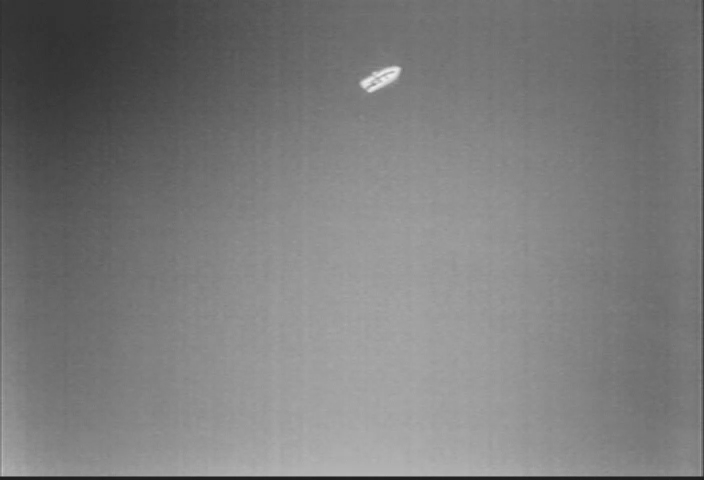
\includegraphics[width=\textwidth]{fig1}
		\caption{caption..}
		\label{fig:2a}
	\end{subfigure}
	~ %add desired spacing between images, e. g. ~, \quad, \qquad, \hfill etc.
	%(or a blank line to force the subfigure onto a new line)
	\begin{subfigure}[b]{0.45\textwidth}
		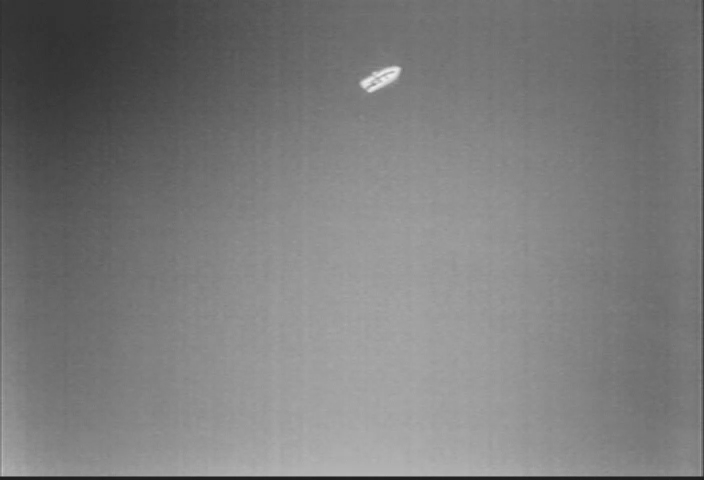
\includegraphics[width=\textwidth]{fig1}
		\caption{caption..}
		\label{fig:2b}
	\end{subfigure}
	\begin{subfigure}[b]{0.45\textwidth}
		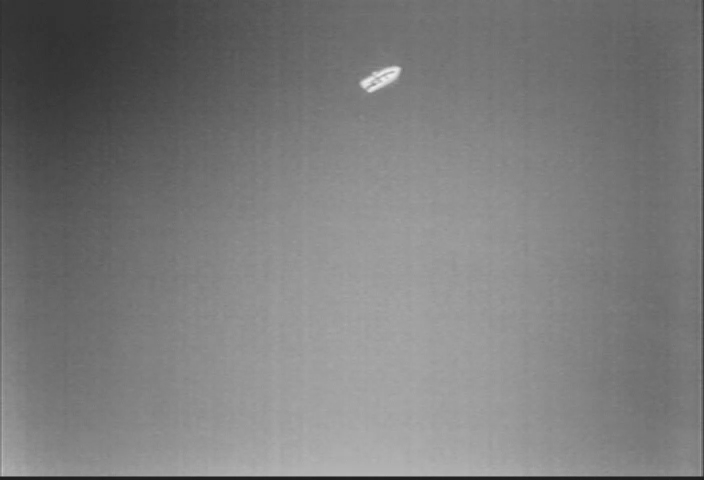
\includegraphics[width=\textwidth]{fig1}
		\caption{caption..}
		\label{fig:2c}
	\end{subfigure}
	\begin{subfigure}[b]{0.45\textwidth}
		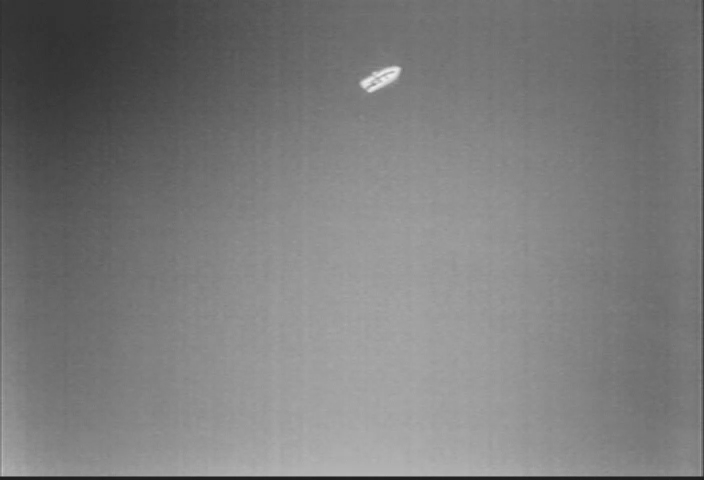
\includegraphics[width=\textwidth]{fig1}
		\caption{caption..}
		\label{fig:2d}
	\end{subfigure}
	\caption{Caption for all figures}\label{fig:2}
\end{figure}
